\documentclass[9pt]{article}
\usepackage[colorlinks=true, allcolors=blue]{hyperref}
\usepackage[table,xcdraw]{xcolor}
\usepackage[utf8]{inputenc}
\usepackage{graphicx}
\usepackage[colorinlistoftodos]{todonotes}
\usepackage[colorlinks=true, allcolors=blue]{hyperref}
\usepackage{multirow}
\usepackage[spanish]{babel}
\selectlanguage{spanish}
% Esto es para poder escribir acentos directamente:
\usepackage[utf8]{inputenc}
\usepackage[T1]{fontenc}
\usepackage{amssymb}
\usepackage{enumitem}
\usepackage{pifont}
\usepackage{tikz}
\usepackage[latin1]{inputenc}
\usepackage{makeidx}
\makeindex
%% Asigna un tamaño a la hoja y los márgenes
\usepackage[a4paper,top=1.2cm,bottom=1.5cm,left=2cm,right=2cm,marginparwidth=1.75cm]{geometry}
\usepackage{wrapfig}
\usepackage{fancyhdr}
\usepackage{multirow}
\usepackage{caption}
\usepackage{longtable}
\usepackage{gensymb}
\usepackage{float}
\usepackage[position=top]{subfig}
\usepackage{verbatim}
\setlength\parindent{0pt}
%% spce line 
\usepackage{setspace}
	\setstretch{1.1}
\usepackage{pdfpages}
%% Paquetes de la AMS
\usepackage{amsmath, amsthm, amsfonts}
\usepackage{tikz}
\usetikzlibrary{shapes.geometric}
\usetikzlibrary{shapes.arrows}
\usepackage{array} 
\usepackage[dvipsnames]{xcolor}
\usepackage{xcolor}
\usepackage{soul}
\newcommand{\mathcolorbox}[2]{\colorbox{#1}{$\displaystyle #2$}}
\date{}

\begin{document}

\begin{titlepage} % Suppresses displaying the page number on the title page and the subsequent page counts as page 1
	\newcommand{\HRule}{\rule{\linewidth}{0.5mm}} % Defines a new command for horizontal lines, change thickness here
	
	\center % Centre everything on the page
	
	%------------------------------------------------
	%	Headings
	%------------------------------------------------
	\includegraphics[width=0.7\textwidth]{logoudesa.jpg}\\[0.8cm]
	
	\textsc{\LARGE Herramietas Computacionales para la Investigación}\\[0.5cm] % Major heading such as course name
	
	\textsc{\Large Amelia Gibbons}\\

	%------------------------------------------------
	%	Title
	%------------------------------------------------
	\textcolor{white}{\HRule}\\[0.6cm]
	\huge\bfseries Trabajo Práctico 2 
	\textcolor{white}{\HRule}\\[1.5cm]
	%------------------------------------------------
	%	Author(s)
	%------------------------------------------------
	\begin{center}
		\Large
		\textsc{Liwski, Sury}\\
	\end{center}
	
	% If you don't want a supervisor, uncomment the two lines below and comment the code above
	%{\large\textit{Author}}\\
	%John \textsc{Smith} % Your name
	
	%------------------------------------------------
	%	Date
	%------------------------------------------------
	\vfill\vfill\vfill % Position the date 3/4 down the remaining page
	{\large 2022}
	\vfill
	
\end{titlepage}
%% acá había una \ y la borré sin querer, no sé para que servía
\section{Chicago - Airbnb 2015 por Comunidad}
\subsection{Mapas}
\subsubsection{Cantidad Airbnbs}
El siguiente mapa muestra como se distribuyen los Airbnbs por cada comunidad de Chicago. Se puede observar que la mayor\'ia se encuentran ubicados en las zonas m\'as c\'entricas, siendo West Town el m\'as poblado por estos. Los bloques son tales que se minimice la varianza en su interior.
\begin{figure}[H]
    \centering
\caption{Mapa de Cantidad Airbnbs por Comunidad 2015}
    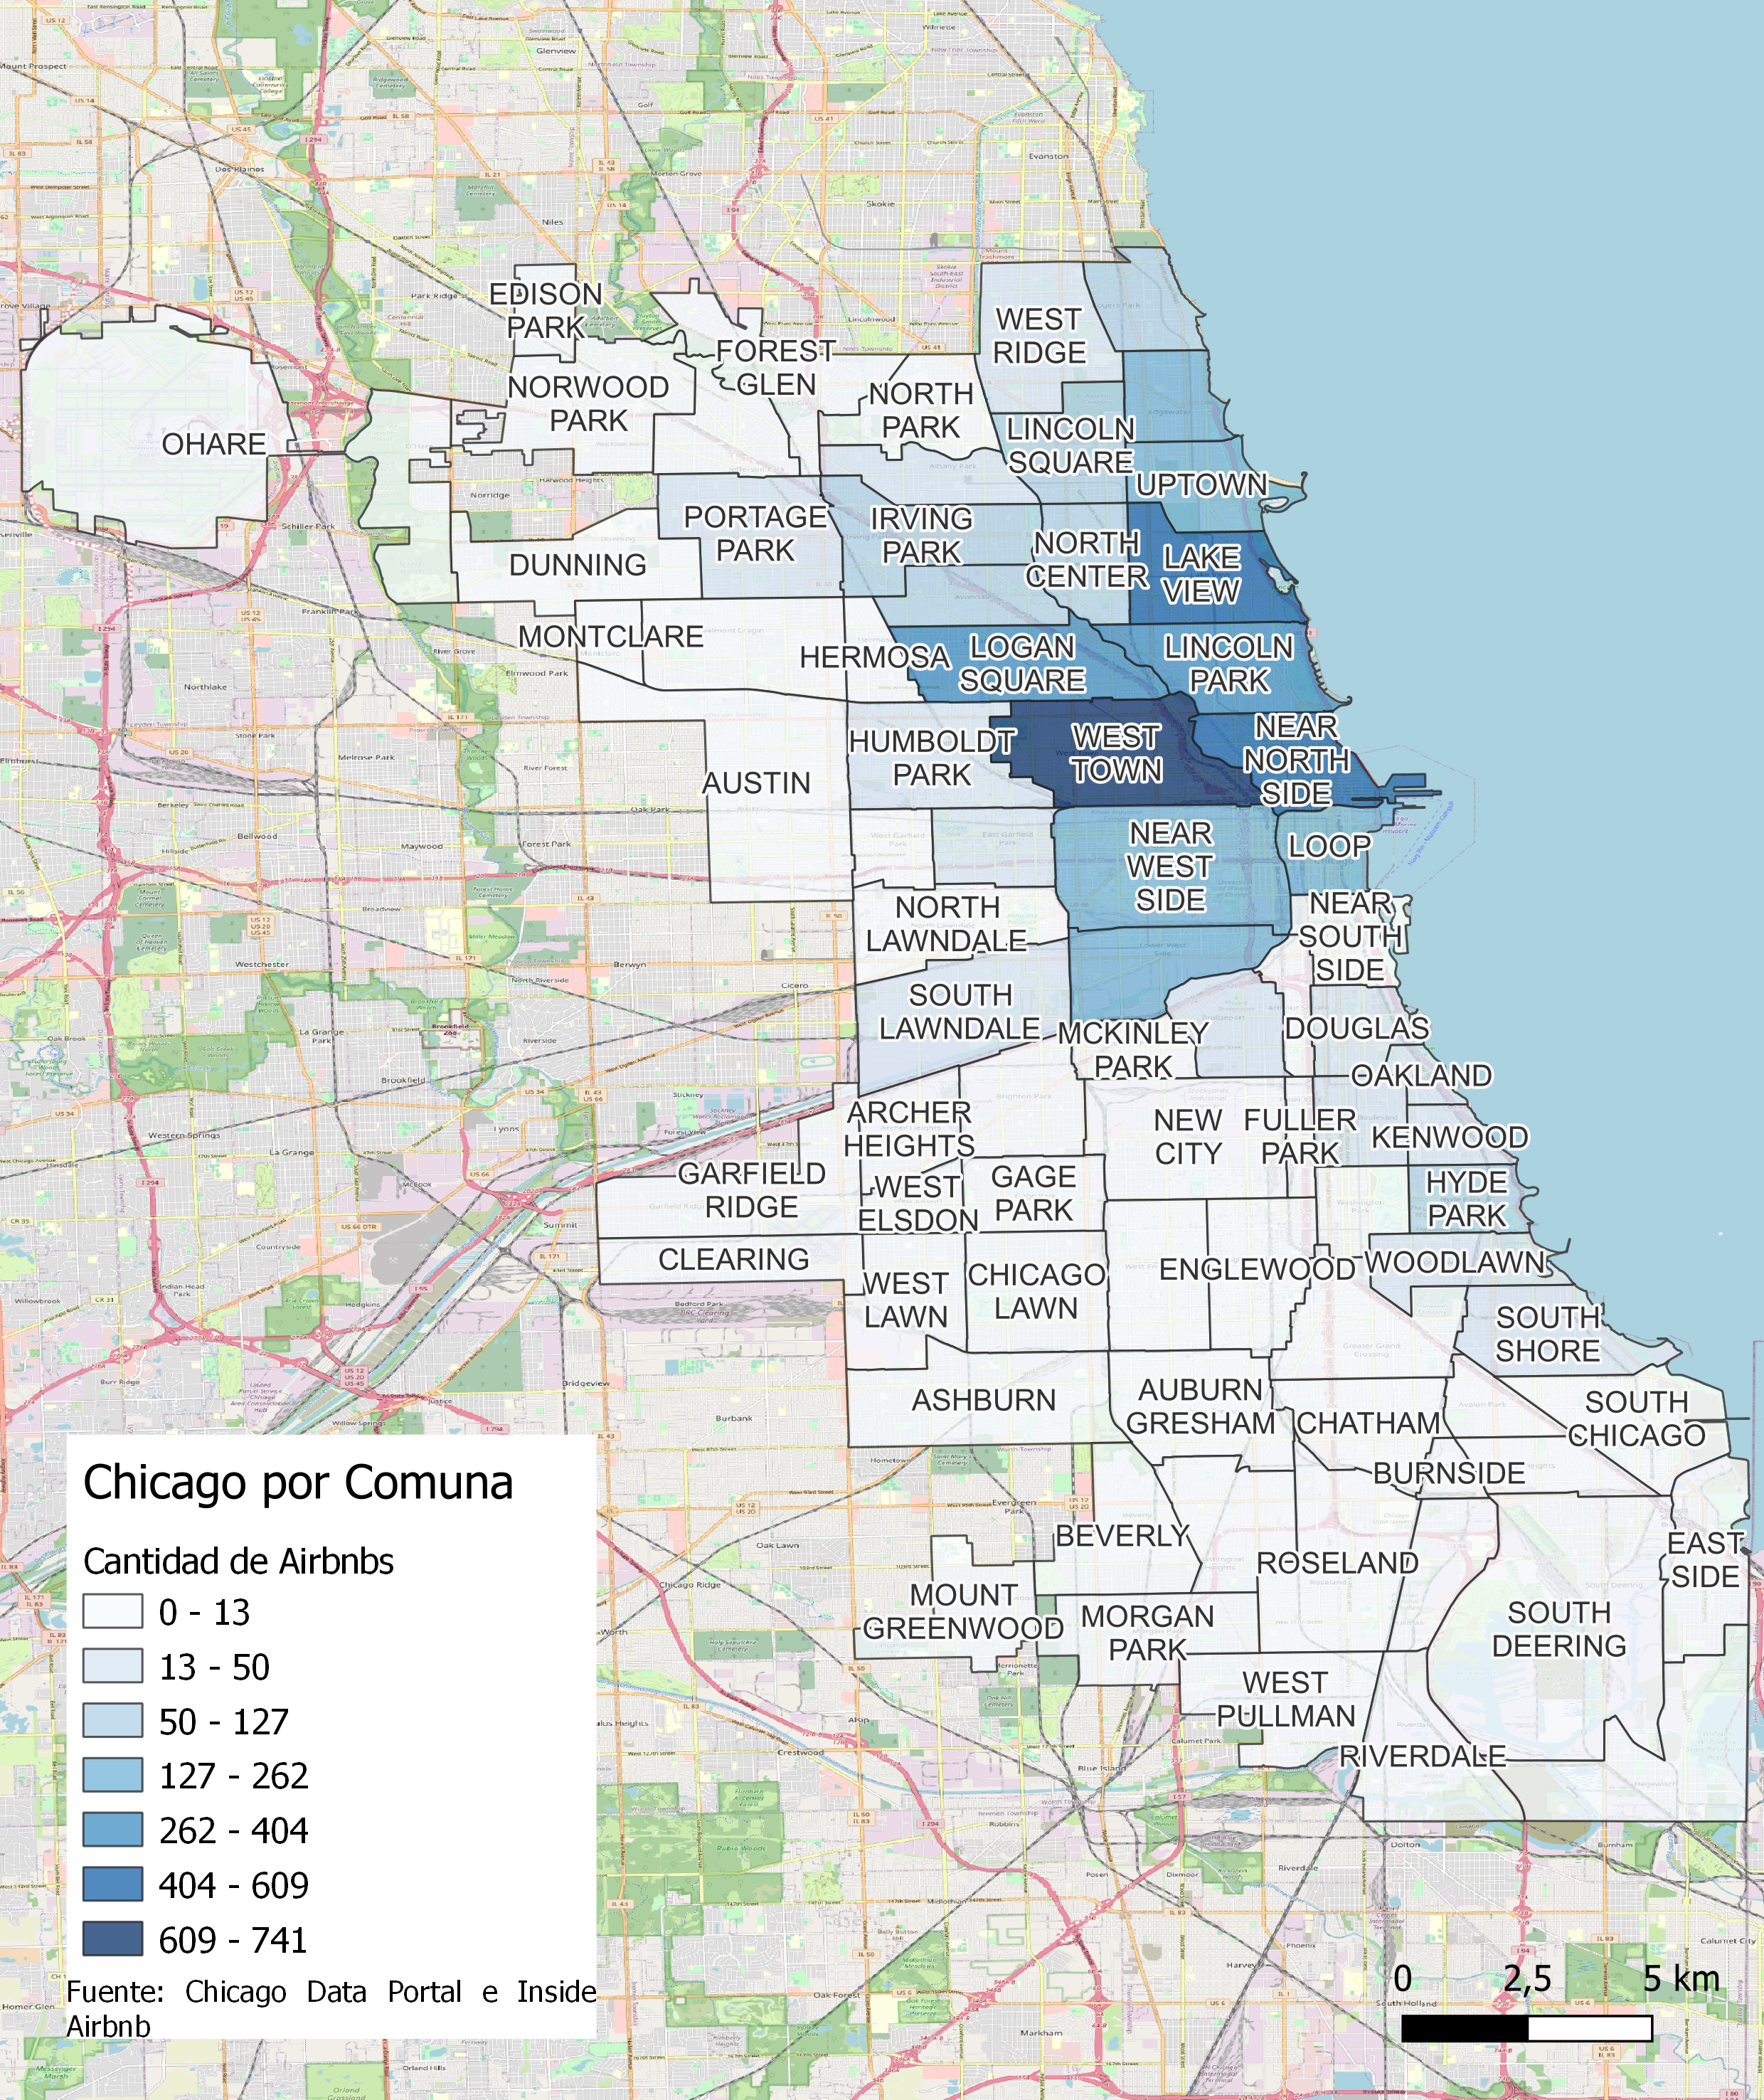
\includegraphics[width=\textwidth]{Graficos Chicago/Cantidad de Airbnb.png}
\end{figure}
\subsubsection{Ingreso per C\'apita}
A continuaci\'on, se encuentra graficado el ingreso per c\'apita promedio de cada \textit{community}. Cuanto m\'as rojo, m\'as bajo es, mientras que verde simboliza que estos sean m\'as altos en promeido. Los bloques son 7, siendo los bloques tales que se minimice la varianza en su interior. Se puede observar que la zona m\'as pobre es en promedio la suroeste y la m\'as rica la noreste 
\begin{figure}[H]
    \centering
\caption{Ingreso per C\'apita Promedio Por Comunidad Chicago 2015}
    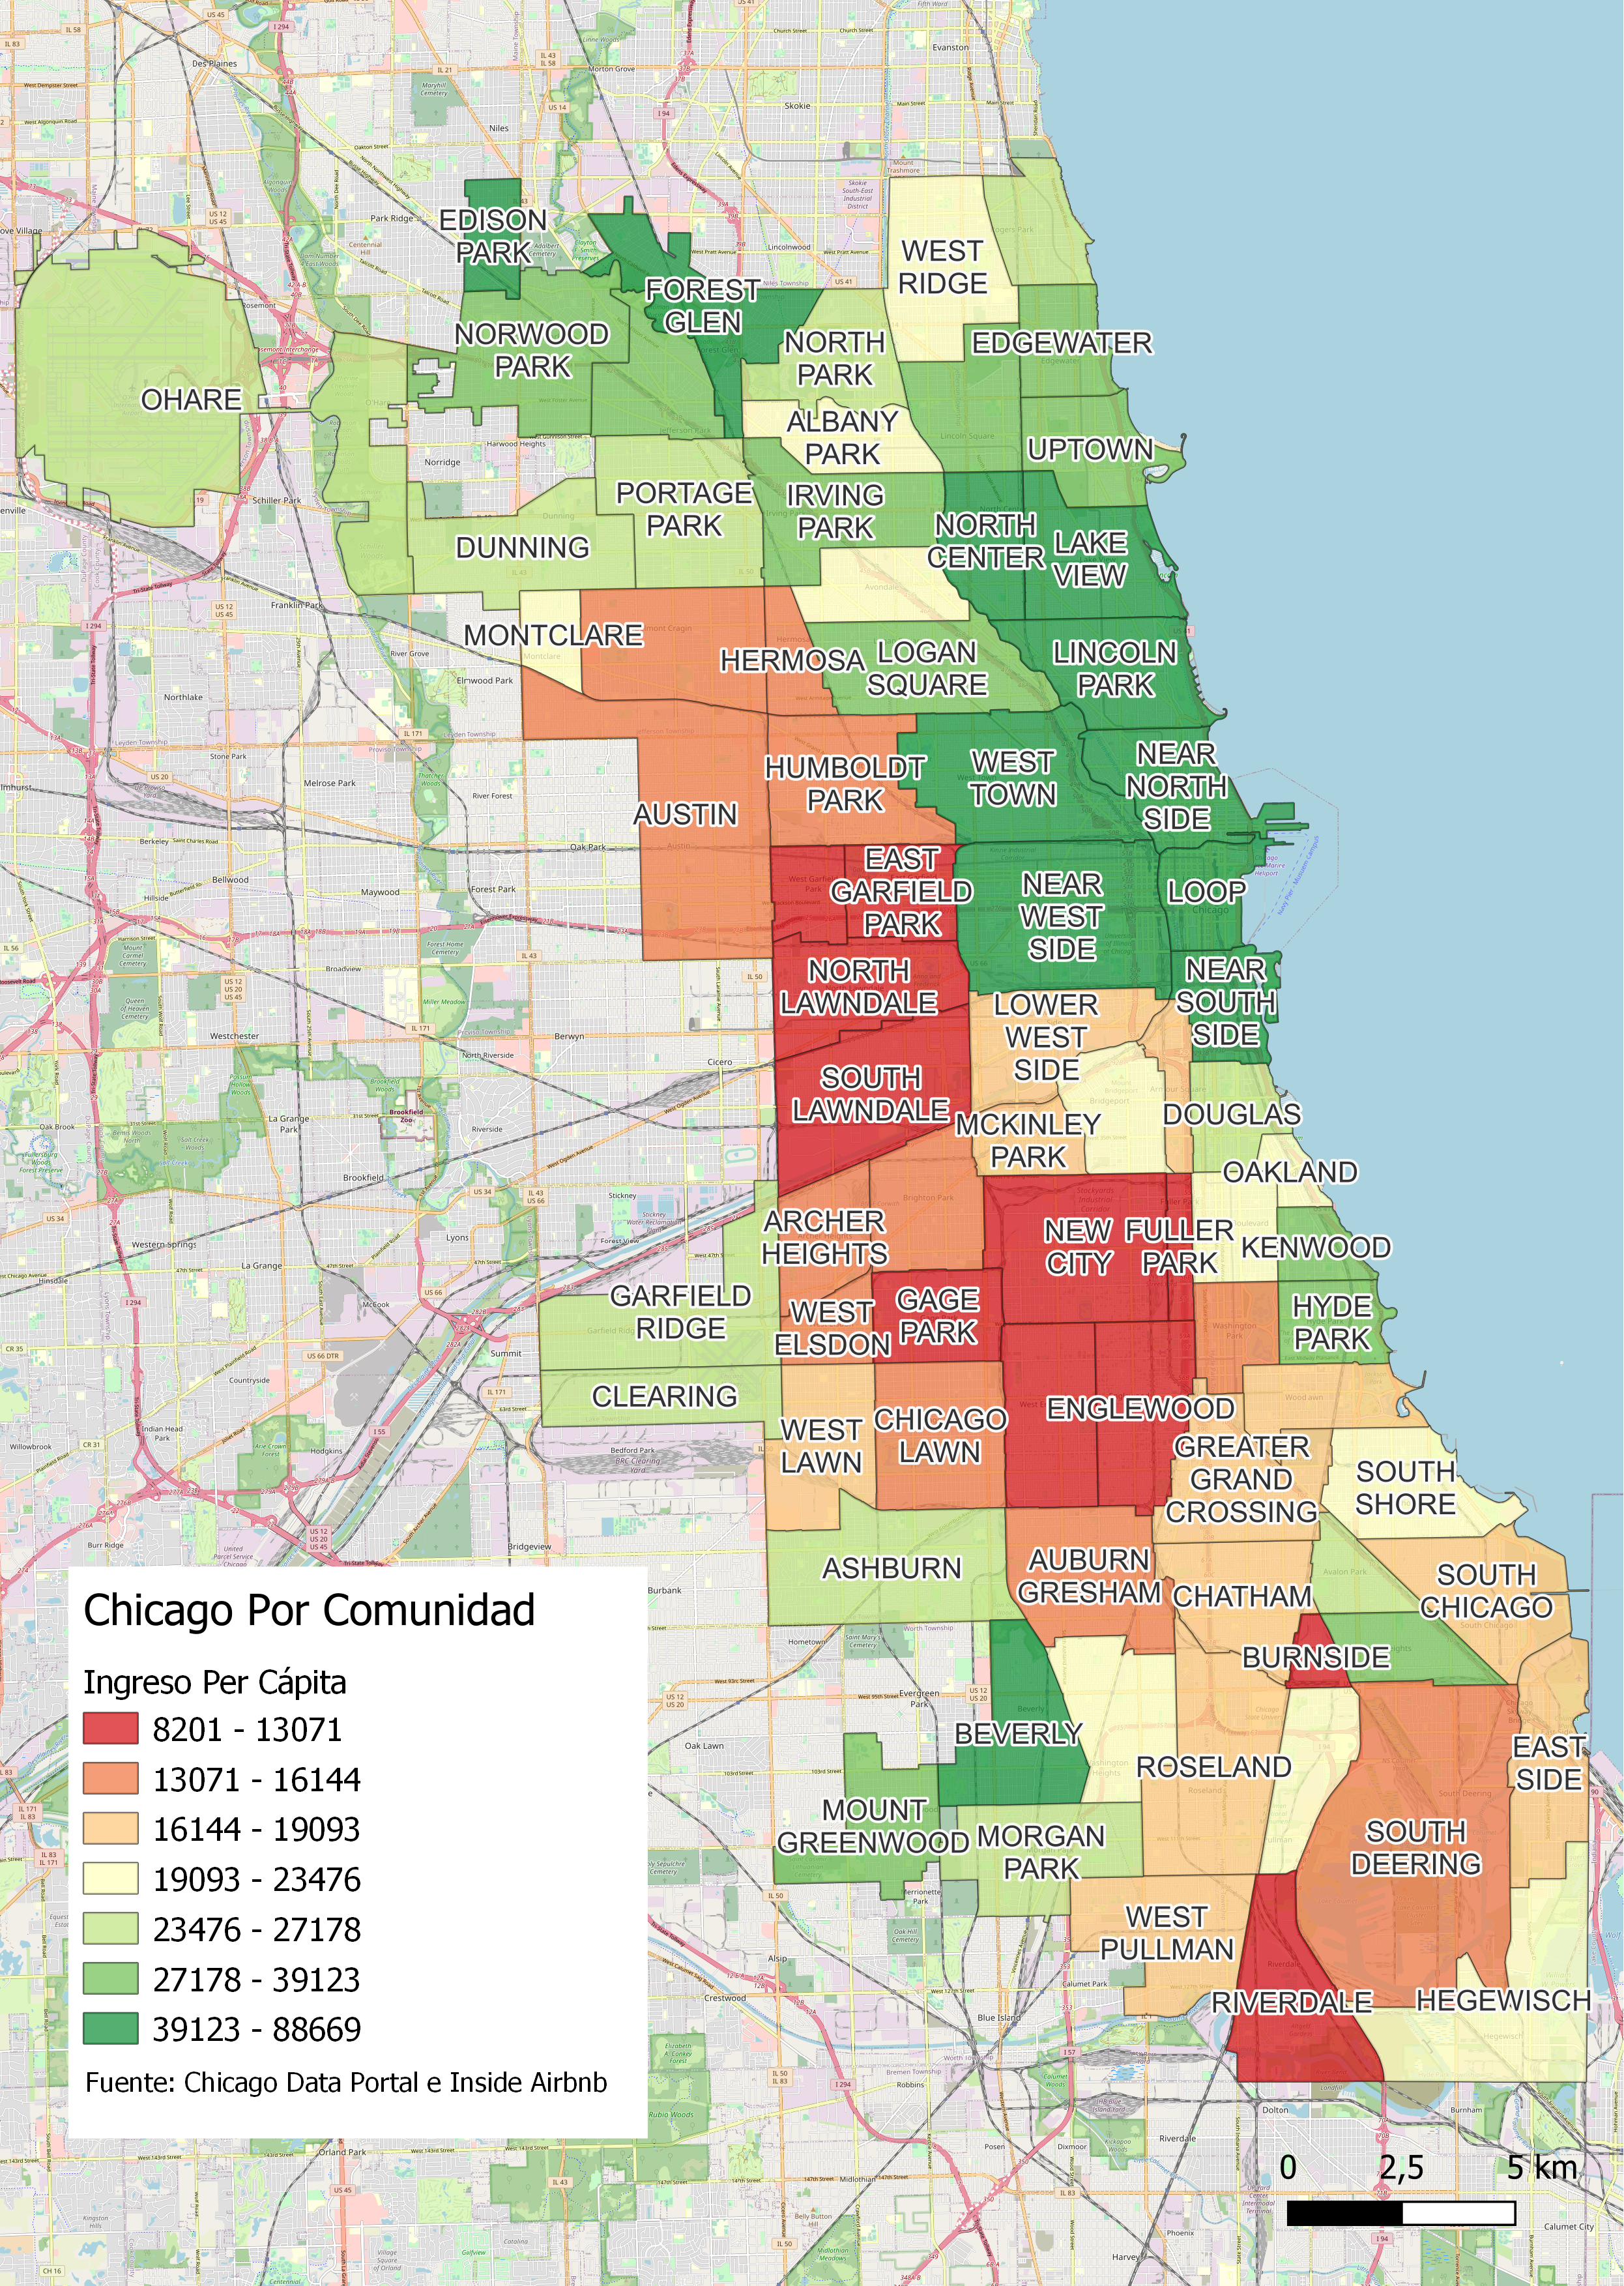
\includegraphics[width=0.9\textwidth]{Graficos Chicago/Income Per Capita.png}
\end{figure}
\subsubsection{Tasa de Desempleo}
Realizando el mismo ordenamiento de bloques de la subsecci\'on anterior, se grafic\'o por comunidad la tasa de desempleo presentada por estas. Se puede observar que son las regiones sur y centro-oeste las que presentan una mayor tasa de desempleo.
\begin{figure}[H]
    \centering
\caption{Tasa de Desempleo Por Comunidad Chicago 2015}
    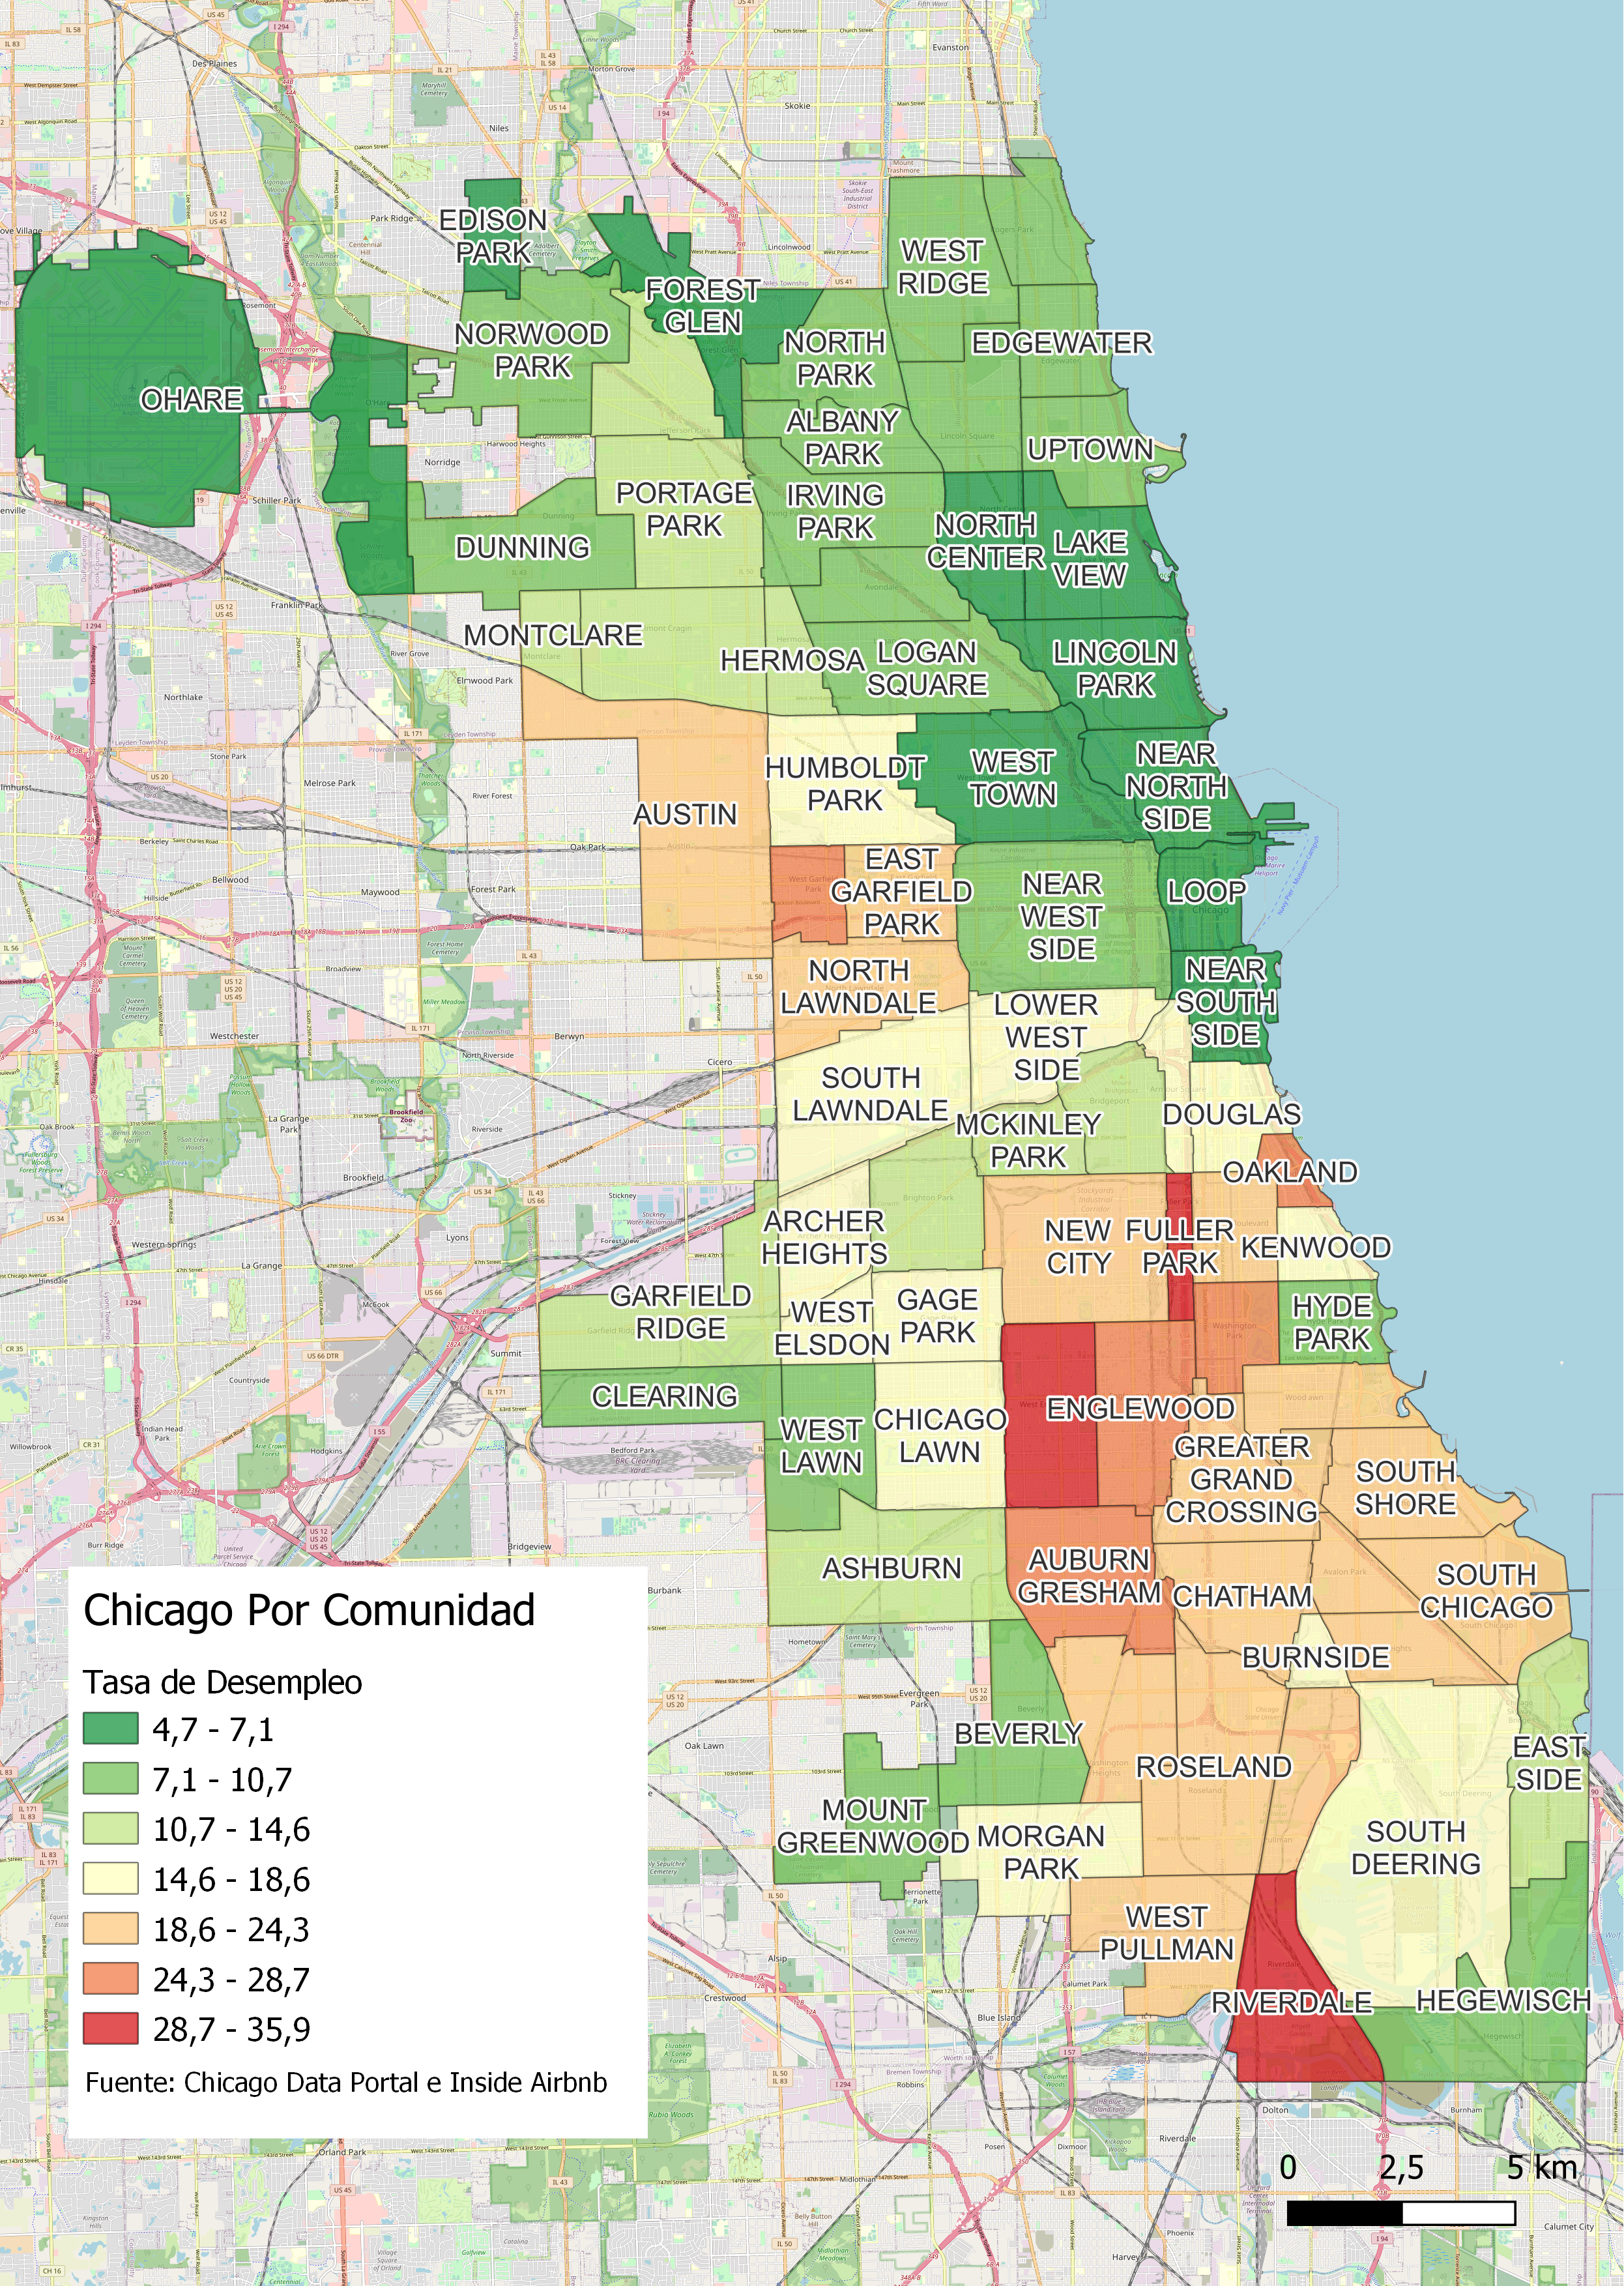
\includegraphics[width=0.9\textwidth]{Graficos Chicago/Tasa de Desempleo.png}
\end{figure}
\subsection{Gr\'aficos}
\subsubsection{Precio Por Persona}
A continuaci\'on se grafica por comunidad el precio por persona. Se puede observar que por lo general se encuentran entre 50 y 100.
\begin{figure}[H]
    \centering

    \includegraphics[width=\textwidth]{Graficos Chicago/prercio por persona.png}
\end{figure}
\subsubsection{Cantidad de Robos vs Tasa de Desempleo}
Con el fin de observar si hab\'ia o no una relaci\'on entre estas dos variables, realizamos el siguiente scatterplot. No hay una clara relaci\'on, aunque llaman la atenci\'on ciertos outliers con bajo desempleo y alta cantidad de robos. Esto podr\'ia ser ya que son comunidades m\'as centricas, habiendo un mayor movimiento de gente, m\'as all\'a de la comunidad en la que vivan. 

\begin{figure}[H]
    \centering

    \includegraphics[width=\textwidth]{Graficos Chicago/Desempleo vs Robos.png}
\end{figure}
\subsubsection{Histograma de Ingresos Per C\'apita}

\begin{figure}[H]
A continuaci\'on se grafica un histograma de frecuencias para el ingreso per c\'apita de cada comunidad. Se puede observar que en su mayot\'ia este es de entre 10000 y 40000 U\$D.
    \centering
\caption*{Histograma Ingreso Per C\'apita}
 
    \includegraphics[width=\textwidth]{Graficos Chicago/Ingreso Per Capita.png}
\end{figure}
\newpage
\section{Buenos Aires}

A continuaci\'on graficamos en un mapa el porcentaje aquellos hogares que presentan al menos un indicador de Necesidades B\'asicas Insatisfechas (NBI). Los datos provienen del Censo Nacional de Población, Hogares y Viviendas del 2010 publicados por el INDEC. Siendo m\'as oscuro un mayor porcentaje, las categorías representan quintiles. El 20\% de los partidos con menos porcentaje de hogares con NBI representa el primer quintil (el m\'as claro), el siguiente 20\% en nivel de NBI representa el segundo quintil, y así sucesivamente, hasta el 20\% con mayor porcentaje de hogares que representa el quinto quintil (el m\'as oscuro). De este modo, puede observarse que los partidos con mayor proporcion de hogares con NBI son los dos m\'as al sur de la provincia y algunos de los primeros cordones del conurbano, pertenecientes al AMBA. 

\begin{figure}[H]
    \centering
    \caption{Porcentaje de hogares con al menos un indicador de NBI por partido de la provincia de Buenos Aires}
    \includegraphics[width=\textwidth]{BSAS_NBI.png}
    \label{fig:NBI}
\end{figure}
\newpage
Luego, graficamos del mismo modo la tasa de desempleo en cada partido. Nuevamente, los datos provienen del Censo Nacional de Población, Hogares y Viviendas del 2010 publicados por el INDEC y han sido clasificados en quintiles. A mayor oscurida, mayor tasa. En relación al mapa anterior, los partidos con mayor porcentaje de hogares con NBI son los que mayor tasa de desempleo presentan, aunque se agregan algunos partidos como General Pueyrred\'on.
\begin{figure}[H]
    \centering
    \caption{Tasa de desempleo por partido de la provincia de Buenos Aires}
    \includegraphics[width=\textwidth]{BSAS_Desempleo.png}
    \label{fig:Desempleo}
\end{figure}


\end{document}
